\begin{figure}[h]
\end{figure}
We repeat the polynomial regression of the previous exercise with the addition of a regularizer (bias). With the use of $bias$ $\lambda$ We tried to regularize my polynomial: basically by summing $\lambda$ We simplify our result while dumping it using a more complex function for regression, so modifying $\lambda$ is conceptually similar to change the degree of the polynomial, offering, however, a greater granularity in the choice of the optimal value.
$\lambda$ represents the level of confidence in the quality of the input data: the more the input is noisier, it is better to use $\lambda$ large and then adopt simple solutions to not fit the noise, the less it is noisy and the more we can decrease $\lambda$ and use more complex solutions in order to fit data.

\begin{figure}[!tbp]

	\centering
	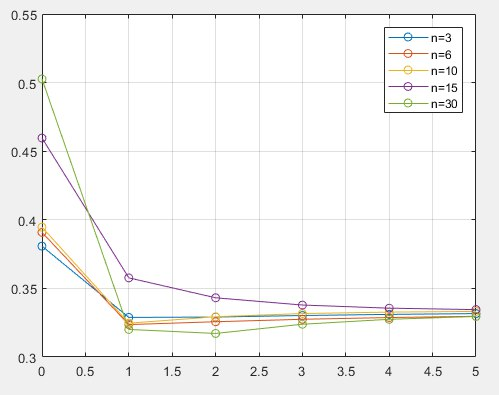
\includegraphics[width=0.45\textwidth]{pl100s10.png}
	\hfill
	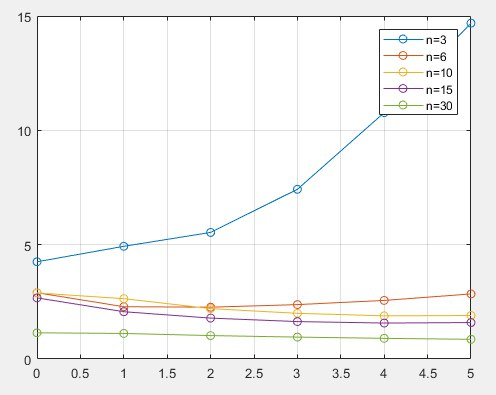
\includegraphics[width=0.45\textwidth]{pl0001s10.png}
\end{figure}
\begin{figure}[!tbp]
	\centering
	\subfloat[fig:lambda = 100 sigma = 10]{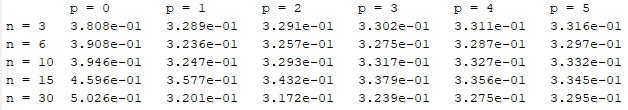
\includegraphics[width=0.45\textwidth]{tl100s10.png}\label{fig:lambda = 100 sigma = 10}}
	\hfill
	\subfloat[fig:lambda = 0,001 sigma = 10]{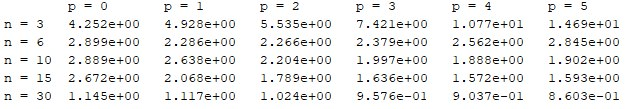
\includegraphics[width=0.45\textwidth]{tl0001s10.png}\label{fig:lambda = 0,001 sigma = 10}}
	
\end{figure}


\begin{figure}[!tbp]
	\centering
	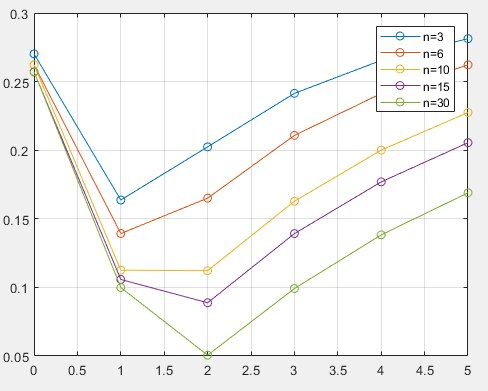
\includegraphics[width=0.45\textwidth]{pl1s001.png}
	\hfill
	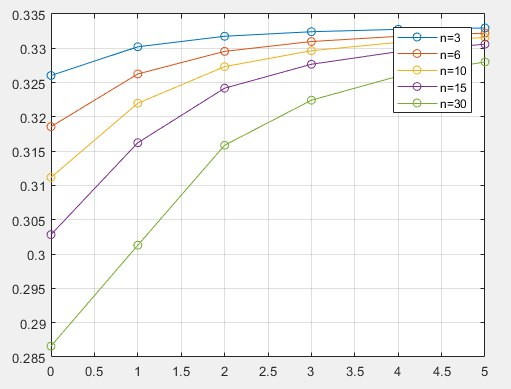
\includegraphics[width=0.45\textwidth]{pl100s01.png}
\end{figure}
\begin{figure}[!tbp]
	\centering
	\subfloat[fig:lambda = 100 sigma = 10]{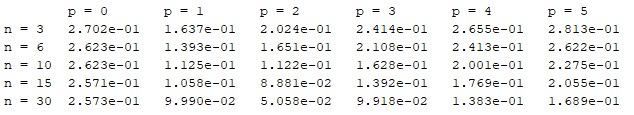
\includegraphics[width=0.45\textwidth]{tl1s001.png}\label{fig:lambda = 1 sigma = 0,01}}
	\hfill
	\subfloat[fig:lambda = 0,001 sigma = 10]{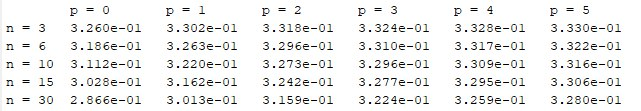
\includegraphics[width=0.45\textwidth]{tl100s01.png}\label{fig:lambda = 100 sigma = 0,01}}
	
\end{figure}






\begin{figure}[h]
	\centering
	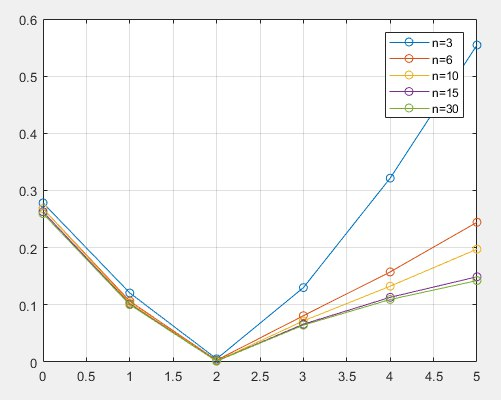
\includegraphics[width=0.5\textwidth]{pl000001s001.png}
\end{figure}

\begin{figure}[h]
	\centering
	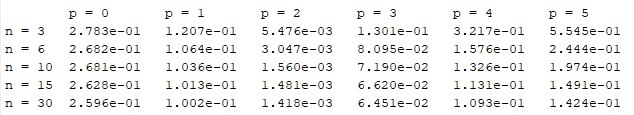
\includegraphics[width=0.5\textwidth]{tl000001s001.png}
	\caption{$\lambda$ = 0,00001 $\sigma$ = 0,01}
	\label{fig:lambda = 0,00001 sigma = 0,01}
\end{figure}